
\begin{resumo}
Esse trabalho descreve o desenvolvimento de um sistema de segurança industrial que requer detecção automática de pessoas. Duas soluções baseadas em imagens de profundidade de visão superior são apresentadas. A primeira é fundamentada em técnicas tradicionais de aprendizado utilizando extração de características e um classificador Support Vector Machine. A segunda utiliza métodos de aprendizado profundo para classificação. A análise de desempenho dos detectores demonstrou que as técnicas profundas têm desempenho superior às tradicionais para esta tarefa entretanto podem oferecer maior custo computacional e necessitar maior conjunto de treinamento.
\end{resumo}

\begin{chave}
Detecção de pessoas, imagens de profundidade, aprendizado profundo, redes convolucionais, aprendizado de máquina, visão computacional.
\end{chave}

\begin{abstract}
This paper describes the development of an industrial safety system that requires automatic human detection. Two solutions based on top-view depth images are presented. The first one is based on traditional learning techniques using feature extraction and a Support Vector Machine classifier. The second solution uses deep learning methods for classification. The performance analysis of both solutions revealed that the deep learning methods outperform traditional learning techniques on this task, at the cost of requiring a larger training set and increased computational cost.
\end{abstract}

\begin{keywords}
  Human detection, depth images, deep learning, convolutional networks, machine learning, computer vision.
\end{keywords}

\section{Introdução}
  Em qualquer ambiente industrial a segurança dos funcionários deve ser garantida. Existem áreas que oferecem maior risco e portanto não devem ser ocupadas durante a operação regular. Um exemplo ilustrativo é de uma fábrica de eletrodomésticos que utiliza uma ponte rolante superior à zona de trabalho para transportar moldes de ferro até máquinas extrusoras de plástico. Esses moldes podem ser pesados e portanto oferecem riscos aos empregados trabalhando sob o chão da fábrica.

  Nesse contexto é útil ter um sistema de segurança automático que detecte pessoas sob o caminho da ponte e interrompa sua movimentação caso encontre uma pessoa. Uma detector baseado em vídeo é ideal nesse caso, especialmente considerando que o ambiente industrial em questão é diversificadamente ocupado por máquinas, moldes e trabalhadores. Como a ponte se movimenta, a câmera deve ser colocada em sua parte inferior, tendo uma vista superior do chão da fábrica. Essas condições impedem que métodos de subtração de fundo (\textit{background subtraction}) sejam utilizados, sendo necessário utilizar algoritmos de detecção mais sofisticados.

  Outro desafio é que as roupas dos trabalhadores não são regulares em cor, e os mesmos não necessariamente usam capacetes ou equipamentos de segurança. Nesse caso, utilizar apenas imagens de cor pode não fornecer informações suficientes para detecção. A fim de superar esse problema, \cite{rauter} usa uma câmera stereo que provê imagens de profundidade dos objetos, oferecendo maior confiabilidade na informação de forma e maior invariância à luminosidade. Essa imagem é então utilizada para localizar candidatos à pessoas, seguido por uma extração de características desenvolvida manualmente e posterior classificação utilizando Support Vector Machine (SVM). Entretanto, esse método pode não oferecer uma solução ideal explicitadas as considerações sobre o ambiente, visto que assume um ambiente limpo e estático, contrário ao ambiente industrial descrito anteriormente.

  Recentemente o aumento do poder computacional, especialmente na forma de \emph{Graphics Processing Units} (GPUs), a disponibilização de grandes datasets de imagens e avanços em métodos de treinamento de redes neurais \cite{nair2010relu} tornou possível um rápido desenvolvimento e uso de métodos profundos de aprendizado nos mais diversos domínios. Ainda, variações densas dessas estruturas permitiram soluções mais eficientes para detecção de objetos \cite{NIPS2013_5207}, complementando resultados anteriores do estado-da-arte em classificação de imagens \cite{hintonCONVNET}. A grande vantagem desses métodos é a mudança de foco da representação de características das amostras, até então desenvolvida manualmente, para um processo automático de representação, requerendo grande quantidade de amostras para oferecer um modelo adequado. Motivado por esses avanços, um segundo método de detecção de pessoas pode ser desenvolvido utilizando imagens de profundidade e classificadores profundos.

  Este trabalho faz uma comparação entre dois métodos de detecção de pessoas, sendo o primeiro ilustrado na Figura \ref{fig:system-diagram}. Ambos utilizam técnicas de visão computacional para detectar candidatos na imagem, descritas na Seção \ref{sec:candidates}. O primeiro detector, baseado em \cite{rauter}, é apresentada na Seção \ref{sec:classical}, enquanto o segundo, utilizando classificadores profundos, é descrita na Seção \ref{sec:deep}. A avaliação quantitativa dos métodos e suas variações é mostrada na Seção \ref{sec:results}. Por fim, conclusões e sugestões de trabalhos futuros são apresentadas na Seção \ref{sec:conclusion}.

  \begin{figure*}[!t]
  \centering
  \includegraphics[width=\linewidth]{system-diagram.png}
  \caption{Diagrama do sistema de detecção de pessoas.}
  \label{fig:system-diagram}
  \end{figure*}

\section{Seleção de Candidatos}
\label{sec:candidates}

    Em um método tradicional de detecção de objetos \cite{traditional-objdetect} o primeiro passo é localizar os candidatos, que são em seguida validados através do processo conjunto de extração de características e classificação. No caso de uma imagem colorida, uma possibilidade para obter candidatos seria utilizar uma janela de tamanho variável que varre a imagem, gerando um candidato a cada deslocamento.

    Entretanto, ao se utilizar imagens de profundidade com visão superior, \cite{rauter} sugere um algoritmo mais eficiente que assume que as pessoas estão entre os objetos mais altos da cena. Apesar dessa hipótese nem sempre ser garantida, ela reduz significantemente o número de candidatos se comparado com o método das janelas deslocadas, e portanto será utilizada nesse trabalho e descrita a seguir.

    Primeiramente, realiza-se a detecção de máximos locais. Divide-se a imagem em blocos de tamanho especificado e cada bloco retorna o pixel com maior intensidade, representando o ponto mais alto naquele bloco. Em seguida, para cada máximo local uma janela quadrada representando o candidato precisa ser obtida. Seu tamanho é calculado como
    %\begin{equation}
      $s_w = \frac{f}{d} \cdot s_r$,
    %\end{equation}
    onde $f$ é a distância focal da câmera, $d$ a distância entre a câmera e o objeto e $s_r$ o tamanho médio da cabeça. A janela de tamanho $s_w$ pixeis é centralizada em torno do respectivo pixel de máximo local.

    O último passo é a centralização da janela sob o candidato utilizando um algoritmo iterativo de \textit{mean shift}. De forma simplificada, esse algoritmo desloca a janela para o centroide dos pixeis dentro dela, de forma que pixeis de maior intensidade tenderão a ficar centralizados sob o candidato.

    A saída desse passo é uma lista de janelas representando os candidatos à pessoas na imagem. Um aspecto relevante a se considerar é o parâmetro de tamanho dos blocos para efetuar a busca de máximos locais. Quando se utiliza blocos muito grandes a probabilidade de ter um objeto muito alto, como uma máquina, no mesmo bloco que uma pessoa é alta, portanto aumenta-se as chances de falha de detecção. Por outro lado, quando se utiliza um bloco muito pequeno, é garantido que todas as pessoas serão consideradas candidatas, porém ao mesmo tempo eleva-se muito o número de candidatos, o que causa um problema de complexidade e desempenho temporal.

\section{Detecção Baseada em Descritores}
\label{sec:classical}

    Após a detecção de candidatos, uma fase de validação é necessária para descartar candidatos que não são pessoas. Uma solução clássica utilizando visão computacional \cite{rauter} utiliza características extraídas por um descritor, desenvolvido manualmente, para alimentar um classificador SVM binário, que retorna uma classe: ``pessoa'' ou ``não-pessoa''. Um descritor de blocos regulares proposto em \cite{rauter} é utilizado. Para aumentar a invariância à rotação, também propomos um descritor de anéis concêntricos (veja Figura \ref{fig:descriptors}). Ambos são descritos a diante, seguidos por mais detalhes do processo de classificação e treinamento.

    \begin{figure}
    \centering
    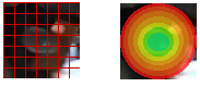
\includegraphics[width=0.9\linewidth]{tradicional/descritores}
    \caption{Descritor de grades regulares (esquerda) e anéis concêntricos (direita).}
    \label{fig:descriptors}
    \end{figure}

    \subsection{Descritor de grades regulares}
      Esse descritor divide a janela do candidato em 7x7 blocos, como ilustra a Figura \ref{fig:descriptors}. O valor médio dos pixeis pertencentes à cada bloco é calculado, gerando uma matriz 7x7 de médias de intensidades de pixeis. Em seguida, o valor do bloco central é subtraído da matriz. Finalmente, calcula-se o histograma da matriz resultante utilizando 32 intervalos. O vetor de histograma, com 32 dimensões, é considerado o vetor de descrição, cuja soma é 49 (número de blocos).

    \subsection{Descritor de anéis concêntricos}
       Primeiramente a janela do candidato é dividida em 18 coroas circulares (ou anéis) cujas distâncias entre os raios internos e externos é constante e cujo centro coincide com o da janela. Então calcula-se a média dos pixeis pertences a cada coroa, resultando num vetor de 18 dimensões. Desse vetor subtrai-se o valor da média dos pixeis da coroa mais interna (cujo raio menor é 0). Por fim, aplica-se a derivada discreta nesse vetor (subtração entre dimensões adjacentes) a fim de enunciar as diferenças entre as médias do pixeis nos diferentes anéis, resultando num vetor de descrição com 17 dimensões.

    \subsection{Classificador SVM}
      Utiliza-se um classificador SVM binário com kernel \textit{Radial Basis Function (RBF)} \cite{rbfkernel} para validar os candidatos. Note que o parâmetro $\sigma$ do kernel, em conjunto com o hiper-parâmetro $C$ do SVM controlam o compromisso entre o desempenho no treinamento e a generalização do modelo em novas amostras. Valores altos de $C$ penalizam erros no conjunto de treinamento, enquanto valores menores priorizam um desempenho melhor no conjunto de teste. O parâmetro $\sigma$ tem efeito similar, porém de maneira inversa. A escolha dos hiper-parâmetros $C$ e $\sigma$ é feita utilizando um processo de validação cruzada com divisão em 5 conjuntos, avaliando a métrica de precisão \cite{evaluationMetrics}.

      Depois de selecionados os hiper-parâmetros, o treinamento final é realizado com todo o conjunto de treinamento. O classificador SVM foi implementado utilizando a biblioteca Scikit-Learn \cite{scikit-learn}.


\section{Detecção Utilizando Aprendizado Profundo}
\label{sec:deep}

    Redes neurais artificiais podem ser utilizadas para uma classificação robusta em diferentes níveis de complexidade, que varia com a estrutura e profundidade da rede. Nós utilizamos e avaliamos duas estruturas de redes profundas: perceptron multi-camadas, ou \textit{multilayer perceptron} (MLP), e redes neurais convolucionais, ou \textit{convolutional neural networks} (CNN). Para ambos os detectores, o candidato é redimensionado para uma janela de 60x60 pixeis e introduzido diretamente ao classificador, sem nenhum processo de extração de características inicial. Podemos considerar que o modelo desenvolve uma representação da amostra a partir das primeiras camadas da rede, sendo que a última camada é responsável pelo processo de classificação e resulta uma única saída interpretada como a probabilidade de o candidato ser uma pessoa. O diagrama dessa abordagem é o mesmo apresentado na Figura \ref{fig:system-diagram} removendo-se o bloco de extração de características e com uma saída probabilística contínua.

    \subsection{Perceptron multi-camadas}
        A estrutura do MLP é composta por unidades organizadas em camadas. Cada unidade pertencente a uma camada está conectada com todas as unidades da camada seguinte. A saída de cada unidade é obtida calculando a soma de suas entradas ponderadas por parâmetros de conexão, seguidas da aplicação de uma função de ativação $\phi(x)$. A informação de cada unidade é propagada de forma direta pela rede desde as camadas de entrada, passando pelas camadas intermediárias até finalmente chegar na camada de saída.

        Utilizamos uma estrutura de 3600 unidades de entrada (60x60 pixeis), 512 e 256 unidades nas camadas intermediárias e uma única unidade de saída, como mostra a Figura \ref{fig:diag-mlp}. Optou-se por essa arquitetura particular pois foi a que empiricamente demonstrou um bom desempenho relativo à complexidade do modelo. As camadas intermediárias, representadas em amarelo, utilizam ativação RELU \cite{nair2010relu} de maneira a evitar o problema de gradiente enfraquecido. A unidade de saída utiliza ativação sigmoide para reproduzir uma saída probabilística.

        \begin{figure}
        \centering
        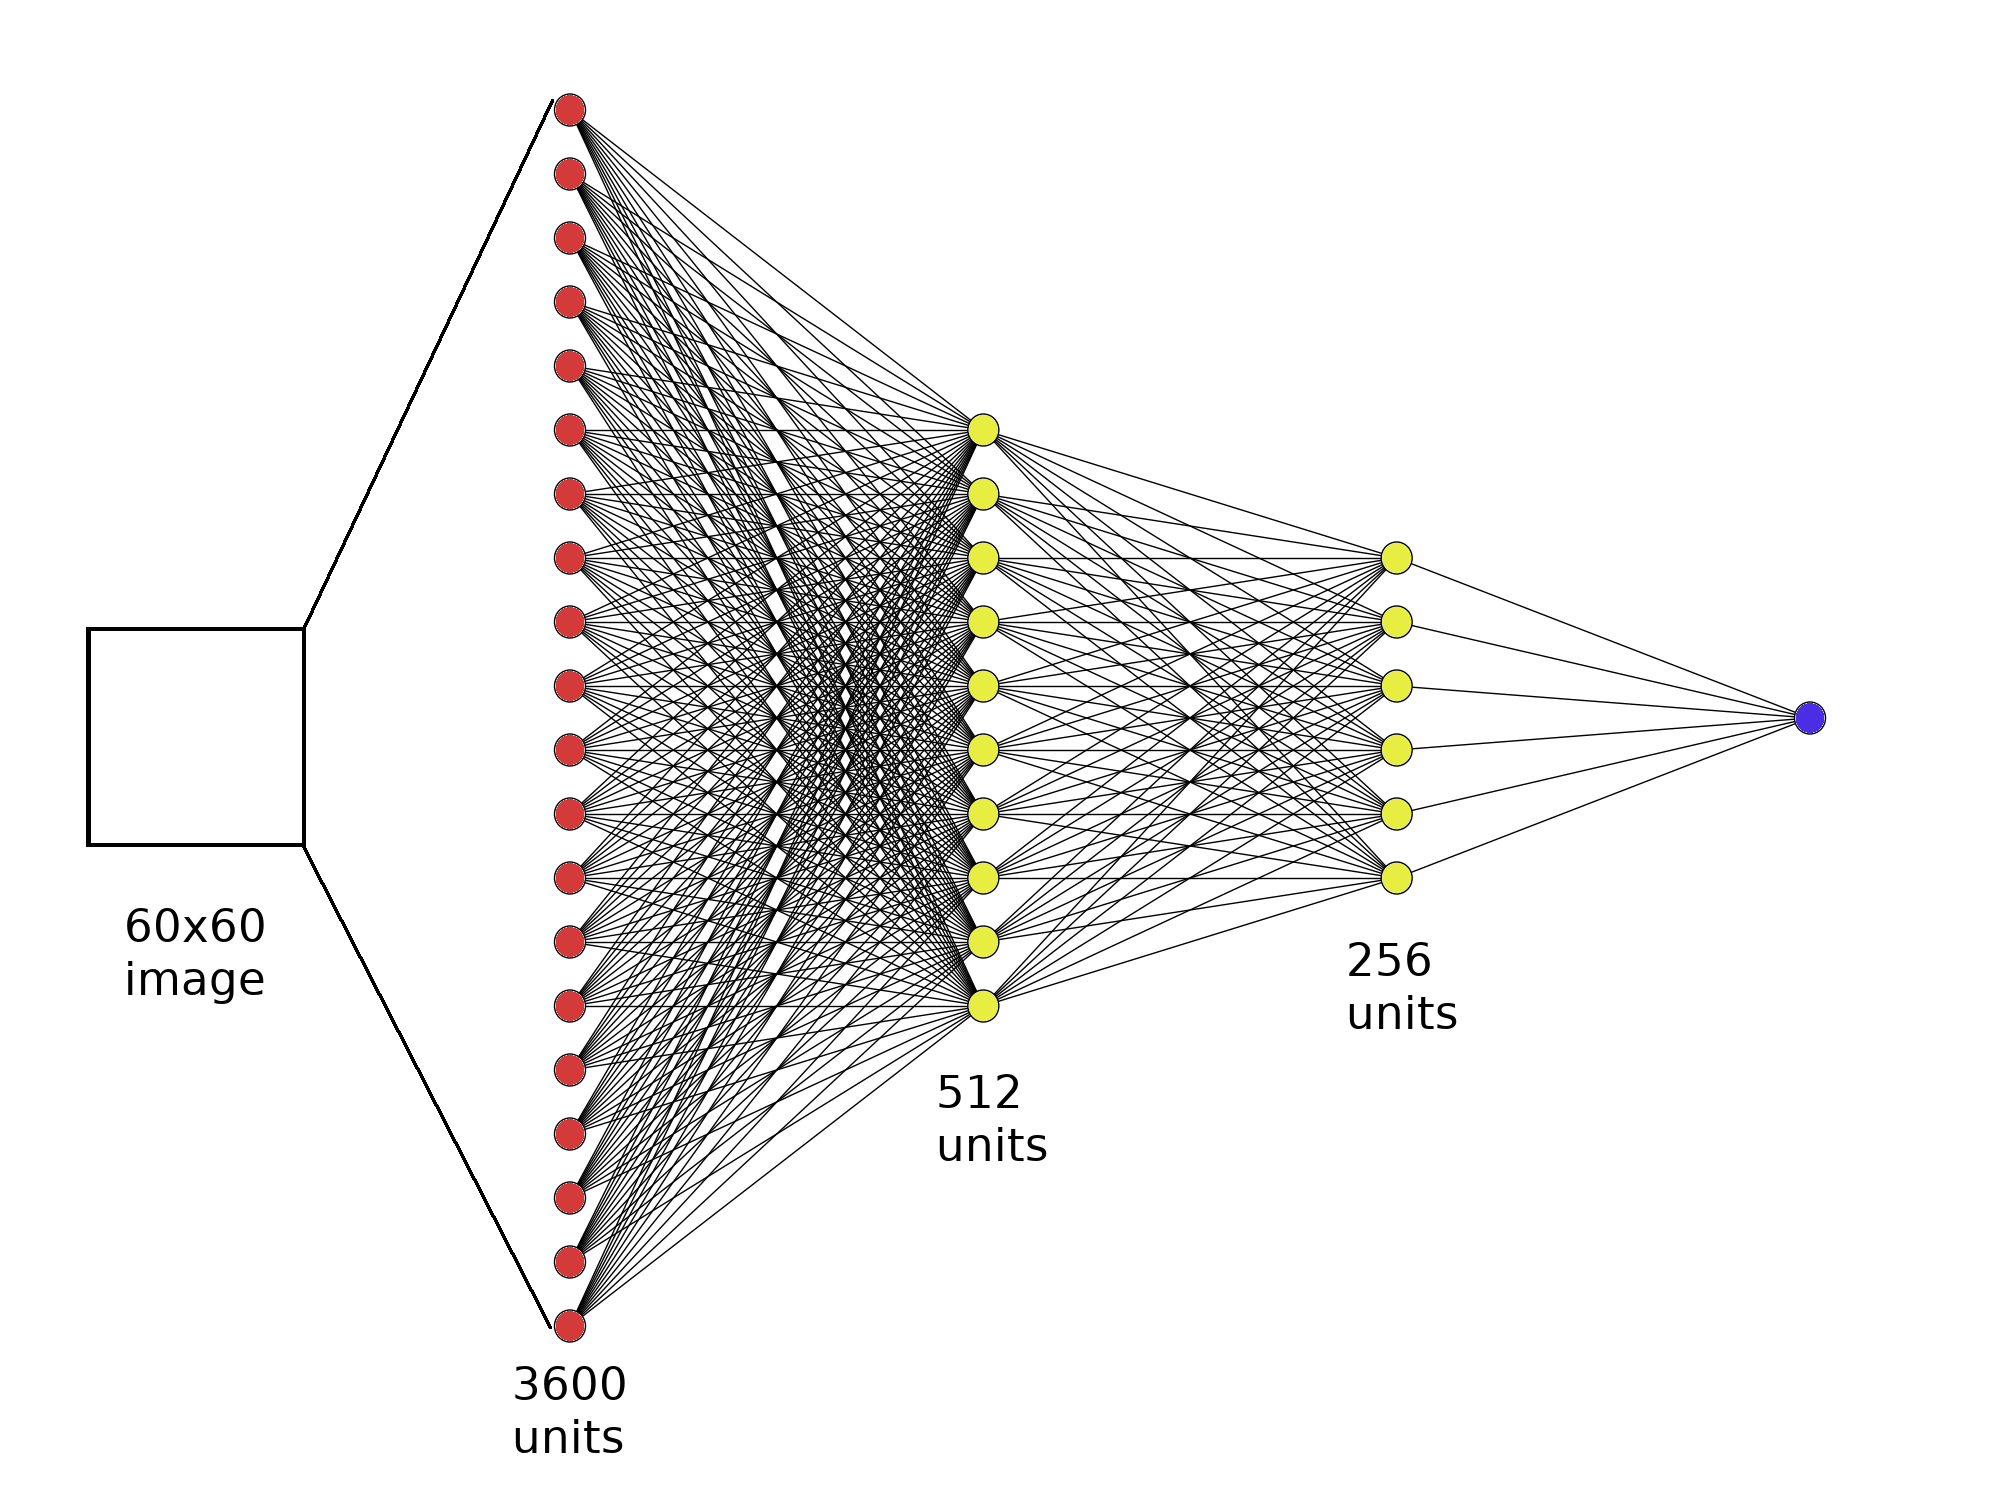
\includegraphics[width=0.8\linewidth]{diagram/diag-mlp.png}
        \caption{Estrutura MLP.}
        \label{fig:diag-mlp}
        \end{figure}

    \subsection{Rede neural convolucional}
         No caso de imagens, existe uma forte correlação entre pixeis de uma redondeza, de forma que não é necessário que cada unidade de uma camada esteja conectada com todas as unidades da próxima camada, mas apenas com alguns pixeis vizinhos. Esse caráter de conectividade local pode ser alcançado através da convolução de uma dada camada com um banco de filtros. Nesse sentido, redes neurais convolucionais podem ser entendidas como uma derivação das MLP e, em geral, fornecem um modelo melhor para imagens através da redução do número de parâmetros e consequente melhora na generalização do modelo.

         Nossa estrutura convolucional, ilustrada na Figura \ref{fig:diag-cnn}, é composta por uma camada convolucional 3x3 com 16 filtros, seguida por uma camada de \textit{max pooling}, e então concatenação resultando em 5776 (16x19x19) unidades seguidas por uma camada densamente ligada de 128 unidades, responsável pela classificação, e única unidade de saída. Novamente, as camadas intermediárias utilizam ativação RELU e a de saída utiliza ativação sigmoide. Optou-se por uma única camada convolucional pelo fato de que uma segunda camada não ofereceu melhora significativa de desempenho.

        \begin{figure}
        \centering
        \includegraphics[width=0.9\linewidth]{diagram/diag-cnn.png}
        \caption{Estrutura convolucional.}
        \label{fig:diag-cnn}
        \end{figure}

    \subsection{Implementação}
        O processo de treinamento consiste na minimização de uma função objetivo, nesse caso, a função de entropia cruzada binária \cite{DLbook}, também conhecida como \textit{logloss}. Seu uso é justificado pela natureza probabilística da camada de saída. O método de otimização é uma variação do \textit{Batch Stochastic Gradient Descent} (B-SGD) chamada Adam \cite{kingma2014adam}, que utiliza uma taxa de aprendizado adaptativa baseada em considerações de momento (do gradiente) para cada parâmetro de otimização.

        Duas formas de regularização foram testadas. Primeiramente utilizou-se L2 com fator 0.01, cujo impacto é diminuir progressivamente o módulo dos pesos do modelo. Observou-se, entretanto, que o desempenho obtido no conjunto de teste foi inferior ao modelo sem regularização. Outra alternativa de regularização testada foi dropout com taxa de 0.5 na camada anterior à classificação. Os resultados se mostraram muito similares ao modelo sem regularização. Optou-se, portanto, por não utilizar regularização, salientando que não foi observado overfitting.

        As tarefas que envolvem visão computacional, extração de candidato e redimensionamento foram realizadas utilizando a biblioteca OpenCV. Ambas as estruturas de classificação profunda foram implementadas utilizando Keras \cite{keras} sob Theano \cite{theano}, que permite utilizar recursos da GPU para efetuar um treinamento rápido, aproximadamente uma época (um passo da iteração, no qual todas as amostras de treinamento são utilizadas uma vez) por minuto.

\section{Resultados}
\label{sec:results}

    A avaliação utiliza as curvas \textit{Receiver Operating Characteristic} (ROC) \cite{evaluationMetrics} para comparar os resultados entre os detectores e seus parâmetros. Essas curvas são geradas através da saída probabilística dos classificadores utilizados. A grande vantagem na natureza probabilística do classificador é a possibilidade de ajustar o compromisso entre as taxas de verdadeiro positivo e falso positivo após treinamento. Isso é feito através da escolha do limiar de probabilidade acima do qual a amostra é considerada positiva (pessoa).

\subsection{Conjunto de dados}
    O conjunto de dados consiste em quatro sequências de vídeo coletadas na fábrica durante um experimento para testar a posição da câmera StereoLabs ZED, fixada na ponte rolante a uma altura de 6m. Todas as sequências foram gravadas pela manhã, com iluminação constante e padrão da fábrica. Cada uma mostra trabalhadores distintos desempenhando suas funções, com ocasional deslocamento da ponte pela fábrica, de maneira que os objetos e máquinas nas cenas se repetem, mas não as pessoas. Selecionam-se duas dessas sequências de vídeo para servirem de base exclusivamente para o conjunto de treinamento e as restantes para o de teste.

    Para formar o conjunto de treinamento selecionam-se as respectivas sequências de vídeo e, para cada quadro, executa-se o algoritmo de seleção de candidatos, manualmente identificando os candidatos como positivos (pessoas) ou não.  Cada amostra é o recorte da janela do candidato sob a imagem de profundidade.

    O conjunto de treinamento utilizado para o SVM é composto por 9894 amostras negativas e 1222 positivas. Para o caso de modelos de aprendizado profundo, que possuem muito mais parâmetros, estendemos o conjunto de treinamento, utilizando mais quadros das sequências reservadas para treinamento, obtendo 14966 amostras negativas e 1932 positivas.

    Uma característica desses conjuntos é a distribuição acentuadamente desbalanceada das classes: no conjunto estendido, por exemplo, mais de 88\% das amostras pertencem à classe negativa. Isso se demonstrou um problema especialmente ao treinar os classificadores profundos visto que a otimização não convergia. Para atacar esse problema utilizou-se ponderação da função custo de forma a penalizar intensamente erros na classe de menor frequência. Todavia, esse método não se mostrou efetivo. Outra tentativa foi a de um balanceamento artifical dos dados. Embora existam maneiras mais sofisticadas para esse fim, tal como gerar novas amostras aplicando transformações de rotação, translação e introdução de ruído a amostras já existentes, optamos por simplesmente replicar as amostras positivas até sua frequência se equiparar às negativas. Mesmo simplista, essa abordagem se mostrou eficiente, permitindo a convergência da otimização ao mesmo tempo em que não se observou overfitting.


    \begin{figure*}
    \centering
    \subfloat[]{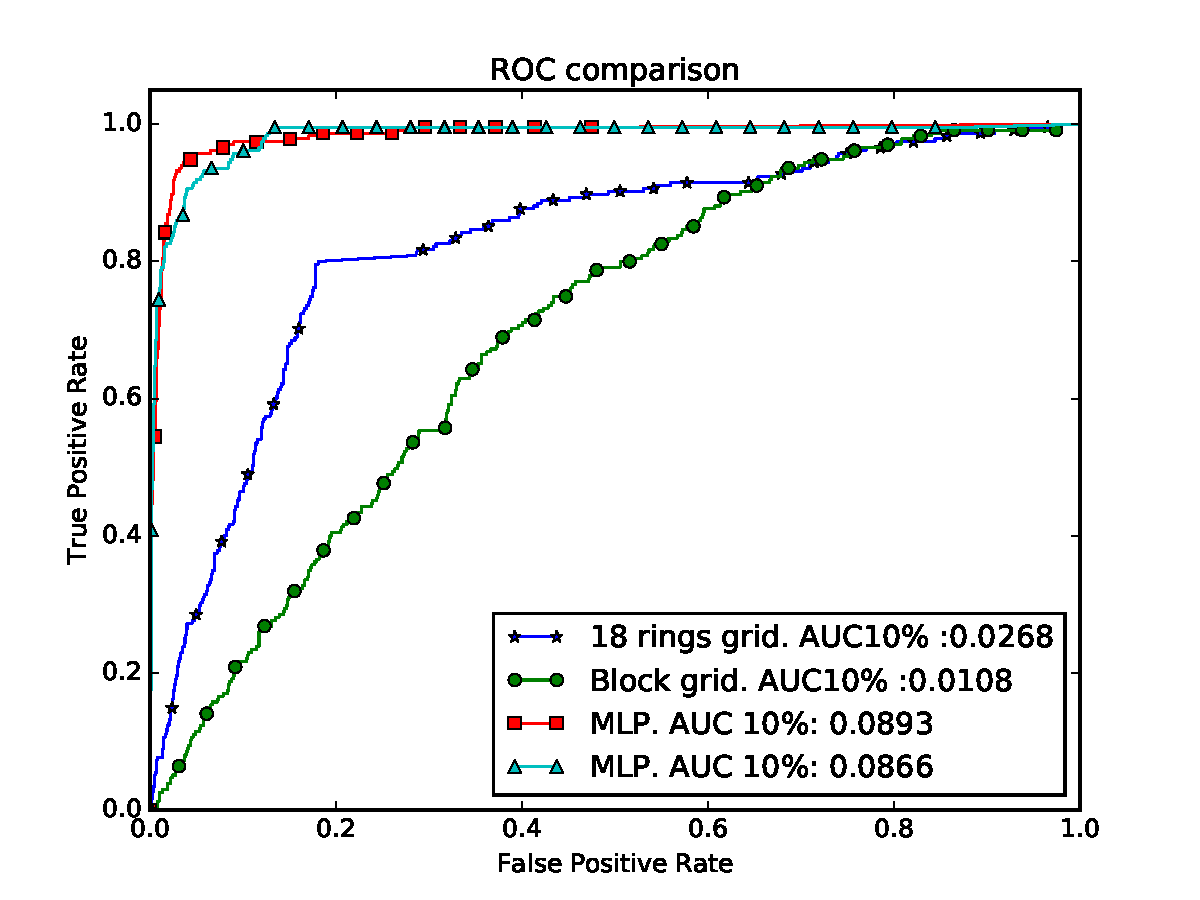
\includegraphics[width=0.45\linewidth]{results/ROC_all.pdf}}%
    \label{fig:result-classifiers-all}
    \hfil
    \subfloat[10 \% zona interesse]{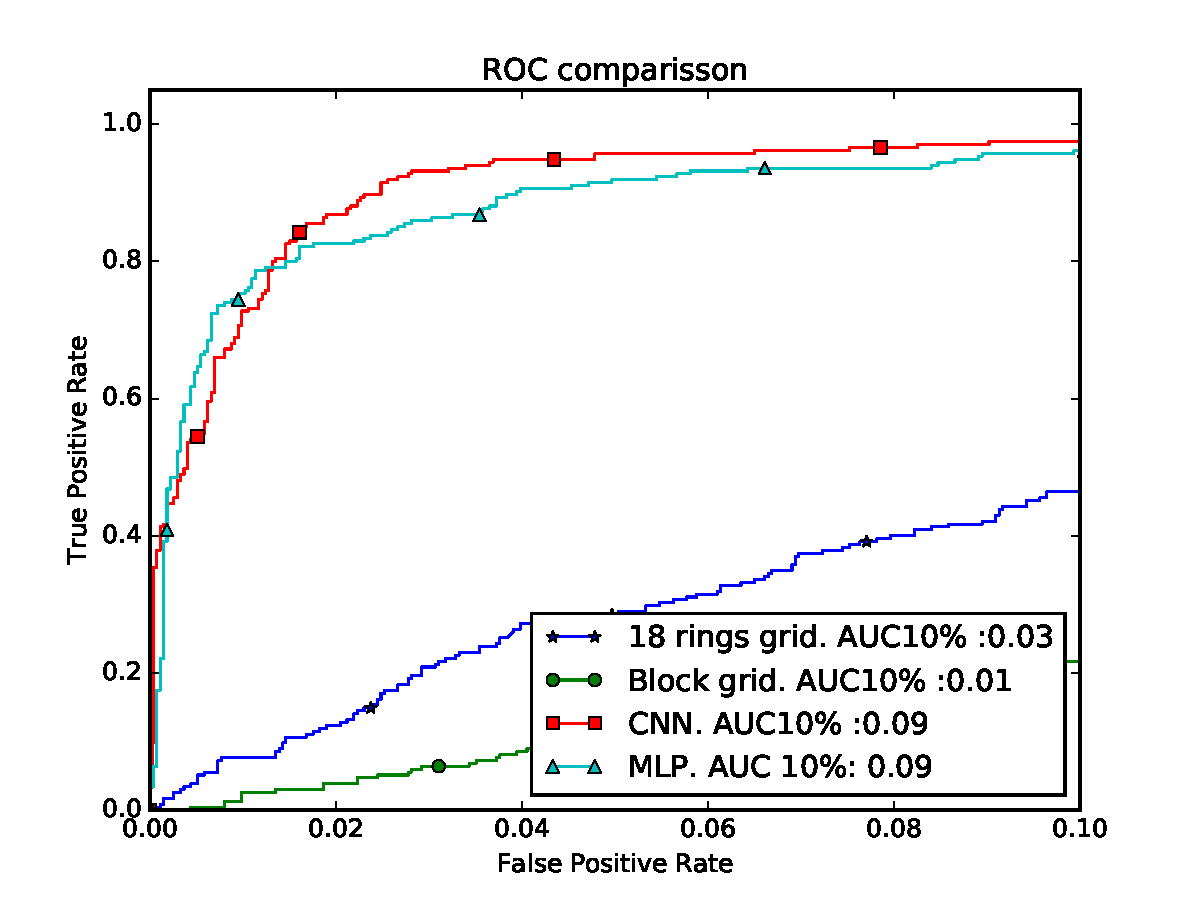
\includegraphics[width=0.45\linewidth]{results/ROC_all_zoom.pdf}}%
    \label{fig:result-classifiers-all-zoom}
    \caption{Desempenho dos classificadores.}
    \label{fig:result-classifiers}
    \end{figure*}


\subsection{Detecção a partir de candidatos previamente extraídos}
    Para avaliar os detectores propostos nas Seções \ref{sec:classical} e \ref{sec:deep}, primeiramente consideramos que os candidatos já foram extraídos das sequência de vídeo reservadas à teste, formando um conjunto de teste com 2738 amostras negativas e 236 positivas. Avalia-se, dessa forma, o descritor (para a abordagem tradicional) e o classificador conjuntamente. A Figura \ref{fig:result-classifiers} mostra o desempenho dos classificadores sob o mesmo conjunto de teste e a métrica \textit{Area Under Curve} (AUC) \cite{evaluationMetrics}. Pode-se observar claramente que os classificadores profundos superam as técnicas tradicionais baseadas na extração de características criadas manualmente. Apesar das estruturas MLP e CNN terem desempenho similares, uma delas pode ser escolhida dependendo da região de operação que se deseja utilizar (maior taxa de verdadeiros-positivos versus menor taxa de falsos-positivos).


    \begin{figure*}
    \vspace{-3ex}
    \centering
    \subfloat[]{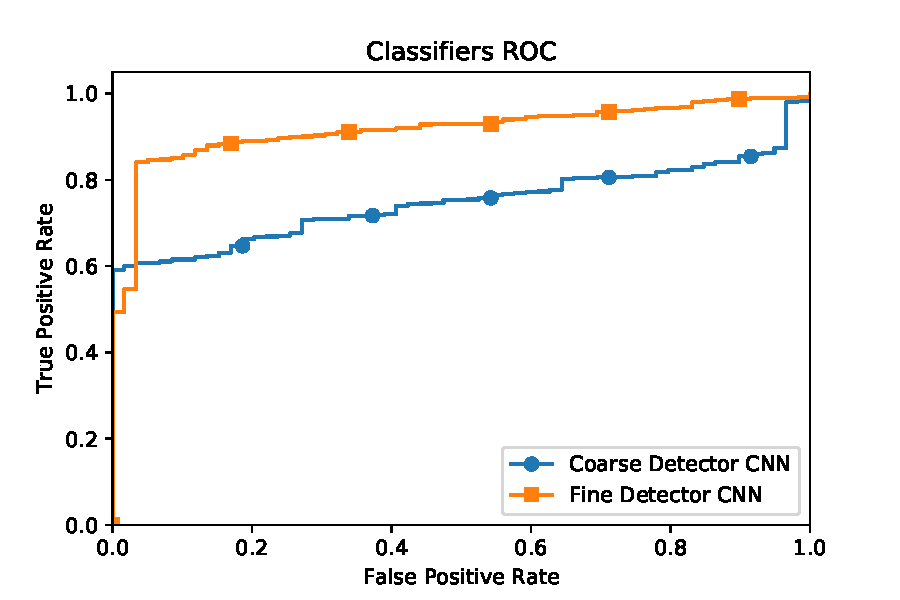
\includegraphics[width=0.45\linewidth]{results/ROC_system.pdf}}%
    \label{fig:result-system-all}
    \hfil
    \subfloat[Zona de interesse de 10\%, melhores resultados]{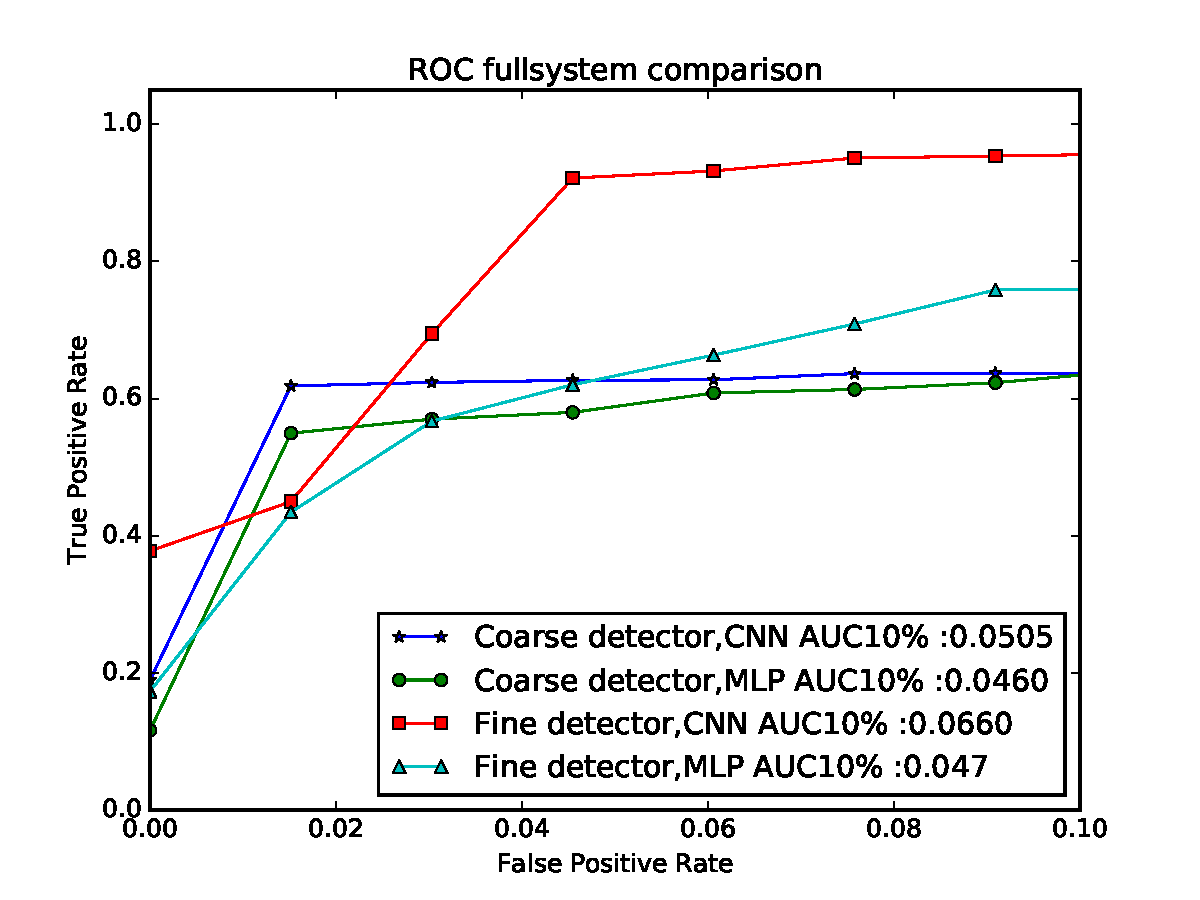
\includegraphics[width=0.45\linewidth]{results/ROC_system_zoom_best.pdf}}%
    \label{fig:result-system-all-zoom}
    \caption{Desempenho global do sistema.}
    \label{fig:result-system}
    \end{figure*}


\subsection{Detecção a partir de quadros completos}
    Em uma segunda etapa consideramos o desempenho global do sistema, incluindo o processo de extração de candidatos. É importante notar que o desempenho observado na Figura \ref{fig:result-classifiers} é um limite superior para o desempenho global, visto que falhas na detecção provenientes da extração de candidatos serão consideradas. Nessa fase o conjunto de teste é composto por quadros inteiros das sequências reservadas para teste, contendo 2336 amostras positivas (frames contendo pessoas) e 64 amostras negativas. A probabilidade de um quadro conter pelo menos uma pessoa é estimada como $1 - \prod_i^n (1-p_i)$ onde $p_i$ é a saída do classificador para o candidato $i$.

    A Figura \ref{fig:result-system} apresenta o desempenho global do sistema utilizando essa formulação com as combinações de classificadores MLP, CNN e diferentes escalas de janelas do processo de extração de candidatos. Os resultados mostram que um para detector grosso (janela grande), o desempenho dos classificadores MLP e CNN são similares, porque os candidatos que são extraídos têm saídas similares. Entretanto, ao utilizar um detector fino (janela menor), muito mais candidatos são detectados, e portanto existe um número maior de amostras para explorar o desempenho desses classificadores, o que permite verificar que o modelo CNN tem desempenho superior ao do MLP.


\section{Conclusão}
\label{sec:conclusion}

    Esse trabalho investiga duas soluções para o problema de detecção de pessoas, uma baseada nas técnicas tradicionais de visão computacional e extração de características manual e outra utilizando métodos de aprendizado profundo. Os resultados apresentados  mostram que o último detector tem desempenho superior ao primeiro, apesar de exigir um conjunto de treinamento maior e oferecer maior custo computacional, portanto requerendo mais poder de processamento. Embora as técnicas de aprendizado profundo sejam consideradas especialmente úteis para grandes conjuntos de dados, nós conseguimos obter um bom resultado mesmo utilizando um conjunto de treinamento de tamanho moderado e desbalanceado.

    Uma possível direção de trabalho futuro é a investigação de um modelo convolucional que não exija uma detecção prévia de candidatos, tendo como entrada o quadro completo e automaticamente identificando regiões de interesse.
